\chapter{Motivating example: smart grid}
\label{chapt:example}
\chapterPage{
In this chapter, we present our motivating example, based on the Luxembourg Smart Grid.
This example has been built in collaboration with our partner, Creos S.A., the Luxembourgish grid manager.
We first several examples of \gls{longTermAct} and then we motivate the need for a language with uncertainty as a first-class citizen with code samples. 
}


%\section{Introduction}

%% Research questions
\paragraph{Delayed actions}
General research question:
\begin{center}
	\textbf{RQ1}: Do current state of the art solutions allow modeling and reasoning over delayed actions?  
\end{center}

Sub research questions:
\begin{itemize}
	\item \textbf{RQ1.1}: How current approaches model the evolution of the context and/or the evolution of the behavior of systems over time?
	\item \textbf{RQ1.2}: Do these solutions model actions, their circumstances and their effects?
	\item \textbf{RQ1.3}: What are the solutions that enable the reasoning over the evolving context and/or behavior of systems?
\end{itemize}


\paragraph{Uncertainty}

%% Methodology
Snowballing approach~\cite{DBLP:conf/ease/Wohlin14}

\paragraph{Inclusion criteria}
\begin{itemize}
	\item \textbf{IC1}: The paper has been published before the May 31 2019
	\item \textbf{IC2}: The paper is available online and written in English
	\item \textbf{IC3}: The paper describes a modeling approach that abstract the context or behavior of a system.
	\item \textbf{IC4}: The paper describes an approach that enables to reason or navigate through a temporal model.
\end{itemize}

\paragraph{Exclusion criteria}
\begin{itemize}
	\item \textbf{EC1}: The paper has less than 4 pages (short paper).
	\item \textbf{EC2}: The paper presents a work in progress (workshop papers), a poster, vision or doctoral studies.
	\item \textbf{EC3}: The paper describes a secondary study (\eg literature reviews, lessons learned).
	\item \textbf{EC4}: The document has not been published in a venue with a peer-review process. For example, technical and research report or white papers.
	\item \textbf{EC5}: The document is an introduction to the proceedings of a venue or a special issue.
\end{itemize}

However, the references of papers rejected are considered for the snowballing iteration.

%\section{Introduction}

%In the previous chapter, we see that the adjustment process of \glspl{adptSyst} can be affected by both uncertain data and \glspl{longTermAct}.
In this chapter, we exemplify the impacts of uncertain data and \glspl{longTermAct} on a \gls{sg} system.
We built these example with Creos Luxembourg, our partner\footnote{Creos Luxembourg is the main grid operator in the country}.
We first give an overview of a \gls{sg}.
Then, we focus on cable load estimation and the impacts of not taking uncertainty into consideration. 
%We find that this case study is particularly appropriate to exemplify the concepts of uncertainty. 
%We highlight and discuss the limitations of existing approaches when handling such scenarios and show how and when our language is superior to these approaches.
Then, we concentrate on the reconfiguration feature of \glspl{sg} and the effect of \gls{longTermAct}.
We also extend this example with other examples from other domain such as cloud infrastructure.

%The remainder of this chapter is as follows.
%We first give an overview of a \gls{sg} in~\Cref{sec:example:sg}.
%Then, we detail our motivating example for \gls{duc} in~\Cref{sec:example:duc} and for \gls{longTermAct} in~\Cref{sec:example:sg}.


\section{Smart grid overview}
\label{sec:example:sg}

\begin{figure*}[ht]
	\centering
    \subfloat[Electricity flow 1] {
		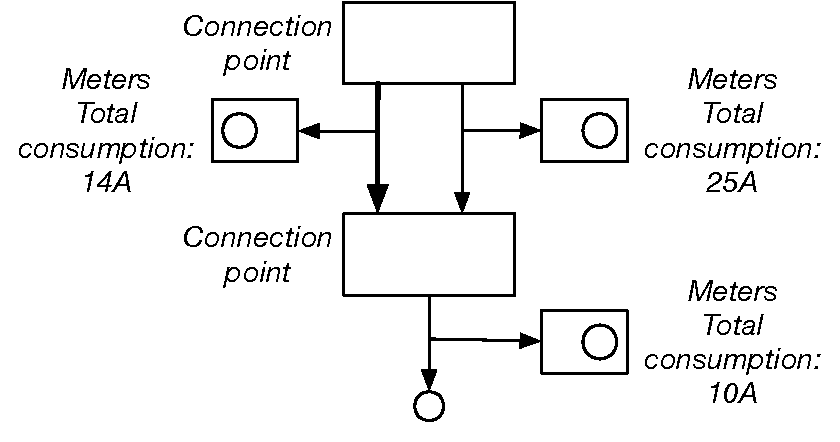
\includegraphics[width=.45\linewidth]{img/chapt-example/duc/Topology1-short}
		\label{fig:intro-schema-topology1}
	}
	\hfill
	\subfloat[Electricity flow 2] {
		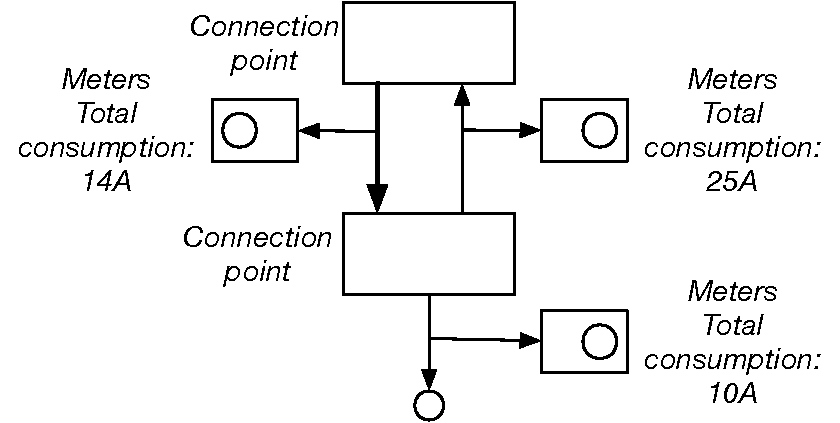
\includegraphics[width=.45\linewidth]{img/chapt-example/duc/Topology2-short}
		\label{fig:intro-schema-topology2}
	}
	\caption{Two different electric flows a same grid topology}
	\label{fig:intro-global}
\end{figure*}

%To exemplify how uncertainty may manifest in programs, we use a smart grid case study, built with Creos Luxembourg, our partner\footnote{Creos Luxembourg is the main grid operator in the country}. 
%More specifically, we focus on cable load estimation and the impacts of not taking uncertain into consideration. 
%We find that this case study is particularly appropriate to exemplify the concepts of uncertainty. 
%We highlight and discuss the limitations of existing approaches when handling such scenarios and show how and when our language is superior to these approaches.

%To exemplify how uncertainty may manifest in programs, we use a smart grid case study, built with a partner Creos Luxembourg\footnote{Creos Luxembourg is the main grid operator in the country. \url{https://www.creos-net.lu}}. 
%We focus on cable load estimation and the impacts of not taking uncertain into consideration. 
%We highlight and discuss the limitations of existing approaches when handling such scenarios.
%Plus, we show how and when our language is superior to these approaches.


%The National Institute of Standards and Technology (NIST) defines a smart grid as ``a planned nationwide network that uses information technology to deliver electricity efficiently, reliably, and securely"\footnote{\url{https://www.nist.gov/engineering-laboratory/smart-grid/smart-grid-beginners-guide}}.
%Conceptually, a smart grid is composed of different entities, like smart meters, cabinets (connection points of cables) and power substations.
%These entities are connected, forming a network, and able to exchange information using different technologies~\cite{DBLP:conf/smartgridcomm/0001FKTPTR14, DBLP:conf/sac/0001MFRKT16}.

%The network is the connection linking the smart grid entities by means of physical cables. 
%Every cable has a maximum load depending on its diameter and the used material.
%Figure~\ref{fig:intro-schema-physical} depicts an example of such a network. 
%This network is composed of one substation, one cabinet, and an arbitrary number of smart meters.
%Every cable has two fuses (to connect or disconnect the cable), one at each endpoint.
%By opening or closing fuses, one can influence the electricity flow through the network.
%Figure~\ref{fig:intro-schema-topology1} and~\ref{fig:intro-schema-topology2} show two possible electricity flows over the same physical network, illustrated in Figure~\ref{fig:intro-schema-physical}. 
%We depict closed fuses in black and the direction of the electricity flow using black arrows.

%Smart meters continuously measure electricity consumption and periodically report it to a central data centre.
%Based on this information, together with the grid topology, the electric load of cables can be computed.
%For example, the load on cable endpoint $i_1$ is equal to $\frac{iL_1 + iL_2 + iL_3}{2}$ in the first configuration and to $iL_1 + iL_2 + iL_3$ in the second one.
%With just one difference in one fuse state, there is a factor 2 of the load on $i_1$ between the two situations.
%If the reader wants to go more into the details of the calculation made, we invite him or her to read~\cite{DBLP:conf/sac/0001MFRKT16}.


Conceptually, a smart grid is a graph where the nodes represent the different entities (like meters, connection points of cables) and the edges represent physical cables.
Every cable has two fuses (to connect or disconnect the cable), one at each endpoint.
By opening or closing fuses, one can influence the electricity flow through the network.
Based on this flow and the electricity consumption, the grid manager can estimate the load in every cable.
This computation is detailed in~\cite{DBLP:conf/sac/0001MFRKT16}.

The flow has a big impact on the load cables.
In \autoref{fig:intro-global}, we depict two different flows for the same grid topology.
In both cases, the measured electric consumption are equal.
However, in \autoref{fig:intro-schema-topology1} the load on the left cable (thick line) equals $\frac{14 + 25 + 10}{2} = 24.5$ whereas it equals $14+25+10=49$ in \autoref{fig:intro-schema-topology2}.
\section[Data uncertainty]{\gls{duc}}
\label{sec:example:duc}

\subsection{Impacts of ignoring data uncertainty} 
\label{subsec:example-possible-consequences}
%Although power grids are becoming more and more automated, today human interventions are still the norm.
%For example, most fuses inside cabinets or substations are manually modified by technicians rather than automatically reconfigured.
%As a consequence, the states of fuses are manually documented by technicians on the field. 
%This of course results in mistakes. 
%One way to address this problem is to take uncertainty into consideration.
%This means considering fuse states as uncertain.
%
%As a consequence, this uncertainty propagates to the load calculation formulas, which depend on the fuse states.
%We call this type of uncertainty \textit{uncertain discrete number}. 
%It also propagates to the final load.
%We refer to these values as \textit{uncertain continuous numbers}. 
%In other words, if the uncertainty of fuse states is not considered, it exists a non-null probability that the observed phenomenon does not reflect the real situation.
%Cable load approximations are used to detect cable overloads and to reconfigure the network if necessary.
%By not considering uncertainty, wrong reconfigurations might be triggered, which could be even worse than if no change would have been applied.
%
%In order to model the electricity flow, we can first use a structure or a class to abstract entities (meter, substation, etc.).
%Then, it can be abstracted by linking different entities.
%For example, the substation in Figure~\ref{fig:intro-schema-topology1} contains two references to the cabinet.
%These references are uncertain due to the uncertain nature of fuse states.
%We refer to these references as \textit{uncertain references}.

Although power grids are becoming more and more automated, today human interventions are still the norm.
For example, most fuses are manually modified by technicians rather than automatically reconfigured.
The states of fuses are thus manually documented by technicians on the field. 
This of course results in mistakes. 
One way to address this problem is to take uncertainty into consideration.
This means considering fuse states as uncertain.

As a consequence, this uncertainty propagates to the load calculation formulas, which depend on the fuse states.
If the uncertainty of fuse states is not considered, it exists a non-null probability that the observed phenomenon does not reflect the real situation.
For example, as we have seen in the previous subsection, a modification of the electricity flow may impact the load of a cable with a factor of 2.
Cable load approximations are used to detect cable overloads and to reconfigure the network if necessary.
By not considering uncertainty, wrong reconfigurations might be triggered, which could worsen the situation.

\subsection{Managing uncertainty is not effortless}
In the following, we describe how uncertainty is commonly handled by application developers using current state-of-the-art approaches. 
We show, through code samples, the limitations of these approaches and why we think that these limitations can be addressed by integrating uncertainty management directly at the language level.
In the code excerpts below, we compute the average cable load over the whole grid based on uncertain cable loads. 
A complete version can be found on the GitHub repository. 
All codes contain at least two classes: \textit{SmartGrid} and \textit{Cable}.
The former contains two fields: an array of Cables named \textit{cables} and a function to compute the average load of cables, named \textit{compute\_avg\_load}.
The latter contains one field: an uncertain number which represents the uncertain load.

\paragraph{Manual implementation} 
%One approach for managing uncertainty is to manually implement all the required features.
%Listing~\ref{lst:example-from-scratch} illustrates this (in Python).
%The excerpt contains three classes, UNumber (lines 1--21), SmartGrid (lines 23--31), and Cable (lines 33--35).
%
%As we can see, this approach comes with several drawbacks.
%First, developers are required to have deep knowledge of probability theory.
%For example, uncertainty can be represented by a normal distribution identified by its mean and variance as shown in the constructor ($\_\_init\_\_$), lines 3 and 4.
%One needs knowledge on how to represent it, how to add two normal distributions, ...
%This type is used in the constructor of the class \textit{Cable} to initialize the cable load (line 28).
%In order to support uncertainty propagation through arithmetic operations, one can think of overloading existing arithmetic operations or defining new ones. 
%Languages like Python and C\# allow operator overloading.
%The method definitions $\_\_plus\_\_$ and $\_\_div\_\_$ overload the '+'  and '/' operations respectively. 
%These operators are later used in the SmartGrid class definition to compute the average load, lines 23 and 25.
%
%Second, manual implementation inevitably increases the size of the code base.
%This will de facto augment the risk of errors in the code.
%Plus, the code will be more difficult to maintain afterwards.
%
%Third, although some languages offer the possibility to overload operators, some typing errors can only be detected at runtime. 
%For instance, since Python is dynamically typed, performing an addition operation between \textit{UNumber} and an \textit{UBoolean} fails and raises an exception only at runtime.
%Whilst, statically typed languages such as C\# can detect such typing errors at development time. 
%Nonetheless, the returned exception message would not be particularly meaningful, as can be seen on the example of  C\#: \textit{Operator `+' cannot be applied to operands of type UNumber and UBoolean}. 
%Handling uncertainty at the language-level and extending the typing system, would significantly improve developers' experience and make it possible to detect typing errors at early stages.

One approach for managing uncertainty is to manually implement all the required features.
Listing~\ref{lst:example-from-scratch} illustrates this in Python.
In addition to the \textit{SmartGrid} and \textit{Cable} class, the excerpt contains an additional one: \textit{UNumber}.

As we can see, this approach comes with several drawbacks.
First, developers are required to have deep knowledge of probability theory.
For example, uncertainty can be represented by a normal distribution identified by its mean and variance as shown in the constructor (\textit{\_\_init\_\_}), line 2.
One needs knowledge on how to represent it, how to add two normal distributions, etc.
For example, here we overload the sum and the division operators for two normal distributions (\textit{\_\_plus\_\_} and \textit{\_\_div\_\_} methods).

Second, manual implementation inevitably increases the size of the code base.
This will de facto augment the risk of errors in the code.
Plus, the code will be more difficult to maintain afterwards.

Third, although some languages offer the possibility to overload operators, some typing errors can only be detected at runtime. 
For instance, since Python is dynamically typed, performing an addition operation between two types of uncertain numbers (\ie represented by two classes) fails and raises an exception only at runtime.
Whilst, statically typed languages such as C\# can detect such typing errors at development time. 
Nonetheless, the returned exception message would not be particularly meaningful, as can be seen on the example of  C\#: \textit{Operator `+' cannot be applied to operands of type UNumber1 and UNumber2}.

%\begin{lstlisting}[style=pythonStyle, caption=Manual management of uncertainty in Python, label=lst:example-from-scratch, linewidth=0.97\textwidth
%]
%class UNumber:
%    def __init__(self, mean=0, variance=0):
%        [...]
%
%    def __add__(self, other):
%       [...] # typing error management + casting other to UNumber if it is a Number
%       return UNumber(self.mean + other.mean, self.variance + other.variance)
%
%    def __div__(self, other):
%       [...] # typing error management + casting other to UNumber if it is a Number
%       value = ((self.mean / other.mean) + 
%             (self.mean * other.variance)) / pow(other.mean, 3)
%       variance = (self.variance / other.mean) +
%             (pow(self.mean, 2) * other.variance) / pow(other.mean, 4)
%       return UNumber(value, variance)
%
%class SmartGrid:
%    def __init__(self):
%        self.cables = []
%
%    def compute_avg_load(self):
%        sum_load = 0
%        for c in self.cables:
%            sum_load += c.load
%        return sum_load / len(self.cables)
%
%class Cable:
%    def __init__(self, id, load=UNumber(0, 0)):
%       [...]
%\end{lstlisting}

\begin{lstlisting}[style=pythonStyle, caption=Manual management of uncertainty in Python, label=lst:example-from-scratch, linewidth=0.97\textwidth
]
class UNumber:
  def __init__(self, mean=0, variance=0):
    [...]
    
  def __add__(self, other):
    [...] # typing error management + casting other to UNumber if it is a Number
    return UNumber(self.mean + other.mean, self.variance + other.variance)
    
  def __div__(self, other):
    [...] # typing error management + casting other to UNumber if it is a Number
    value = ((self.mean/other.mean) + (self.mean*other.variance)) / pow(other.mean, 3)
    variance = (self.variance / other.mean) +
             (pow(self.mean, 2) * other.variance) / pow(other.mean, 4)
    return UNumber(value, variance)

class SmartGrid:
  [...]
  def compute_avg_load(self):
    sum_load = 0
    for c in self.cables:
      sum_load += c.load
    return sum_load / len(self.cables)
    
class Cable:
  def __init__(self, id, load=UNumber(0, 0)):
    [...]
\end{lstlisting}

\paragraph{Using existing libraries for probability theory}
%Since uncertainty management relies on probability theory, another approach is using a library implementing common probability distributions.
%%\footnote{\url{https://docs.scipy.org/doc/scipy/reference/stats.html}}
%Staying in Python, there is a widely used library called SciPy library\footnote{\url{https://www.scipy.org/}} and in particular the \textit{stats} module, defining different probability distributions, e.g. the Bernoulli and the Gaussian distributions (cf. Section~\ref{sec:data-uncertainty}).
%Whereas these libraries are suitable to compute different properties of probability distributions, it remains the responsibility of developers to define how to perform arithmetic operations on distributions.
%Listing~\ref{lst:limit-lib-proba} shows an example of the definition of the\textit{ add\_gaussian} method, responsible for adding up two uncertain numbers represented as Gaussian distributions. 
%
%Using such libraries does not prevent developers to have a deep understanding of the probability theory.
%They have been designed to help them manipulating probability distributions, but they still required knowledge about them.
%For example, as shown in Listing~\ref{lst:limit-lib-proba}, one may access the mean and the variance of a normal distribution.
%However, she or he needs to know how two normal distributions can be added.
%This also increases the code base and thus is prone to errors.
%Finally, as it is a library, typing errors will still remain either detected at runtime or not helpful for developers.
Since uncertainty management relies on probability theory, another approach is using a library implementing common probability distributions.
%\footnote{\url{https://docs.scipy.org/doc/scipy/reference/stats.html}}
Staying in Python, there is a widely used library called SciPy\footnote{\url{https://www.scipy.org/}} and in particular the \textit{stats} module, defining different probability distributions.
Whereas these libraries are suitable to compute different properties of probability distributions, it remains the responsibility of developers to define how to perform arithmetic operations on distributions, as depicted in \autoref{lst:limit-lib-proba}.

Using such libraries does not prevent developers to have a deep understanding of the probability theory.
They have been designed to help them manipulating probability distributions, but they still required knowledge about them.
For example, as shown in Listing~\ref{lst:limit-lib-proba}, one may access the mean and the variance of a normal distribution.
However, she or he needs to know how two normal distributions can be added.
This also increases the code base and thus is prone to errors.
Finally, as it is a library, typing errors will still remain either detected at runtime or not helpful for developers.


%\begin{lstlisting}[style=pythonStyle, caption=Limitation using a probability library (Python), label=lst:limit-lib-proba, linewidth=0.97\textwidth]
%from scipy.stats import norm
%
%def add_gaussian(g1, g2):
%    [...]
%    return norm(g1.mean() + g2.mean(), g1.var() + g2.var())
%
%def div_gaussian(g1, g2):
%   [...]
%
%class SmartGrid:
%    def __init__(self):
%        self.cables = []
%
%    def compute_avg_load(self):
%        sum_load = 0
%        for c in self.cables:
%            sum_load = add_gaussian(sum_load, c.load)
%        return div_gaussian(sum_load, len(self.cables))
%
%class Cable:
%    def __init__(self, id, load=norm(0, 0)):
%        [...]
%\end{lstlisting}

\begin{lstlisting}[style=pythonStyle, caption=Limitation using a probability library (Python), label=lst:limit-lib-proba, linewidth=0.97\textwidth]
from scipy.stats import norm

def add_gaussian(g1, g2):
    [...]
    return norm(g1.mean() + g2.mean(), g1.var() + g2.var())

def div_gaussian(g1, g2):
   [...]

class SmartGrid:
    [...]
    def compute_avg_load(self):
        sum_load = 0
        for c in self.cables:
            sum_load = add_gaussian(sum_load, c.load)
        return div_gaussian(sum_load, len(self.cables))

class Cable:
    def __init__(self, id, load=norm(0, 0)):
        [...]
\end{lstlisting}

\paragraph{Using existing libraries for uncertainty}
%Another commonly used approach is to use existing libraries for data uncertainty.
%For example, in Python, using the \textit{uncertainties~\cite{url:uncertainties} library}, a developer can manipulate uncertain floats using variables of type \textit{ufloat}.
%The uncertainty propagation is handled transparently.
%In Listing~\ref{lst:example-python-uncertainties}, we depict a minimalistic excerpt of the necessary code to compute the mean load using an existing library for data uncertainty.
%Unlike the previous code snippet, this listing contains only two classes, SmartGrid and Cable.
%Moreover, the cable load property initialization uses \textit{ufloat} instead of \textit{UNumber}.
%
%Using a library can tackle the two first drawbacks existing in the previous approach: required knowledge of probability theory and code complexity.
%Indeed, the implementation of the probability theory is encapsulated inside the library.
%Developers will just use it through its API.
%The complexity of the implementation, with the possible errors, are also pushed to the complexity.
%We can argue that the library will be well tested and documented.
%
%However, similarly to the previous example, this approach does not extend the type system.
%If the language relies on a dynamic type system (like in Python), then typing errors are raised only at runtime.
%In any case, raised exceptions are not very meaningful.
%For example, if two distributions are sum whereas the operator has not been overloaded for the input distributions, then the error message will just state this operation is not implemented, without any more information.
Another commonly used approach is to use existing libraries for data uncertainty.
For example, in Python, using the \textit{uncertainties}~\cite{url:uncertainties} library, a developer can manipulate uncertain floats using variables of type \textit{ufloat}.
The uncertainty propagation is handled transparently.
In Listing~\ref{lst:example-python-uncertainties}, we depict the code of the load average computation using this library.
The only difference from the previous code snippet, is the missing of the \textit{UNumber} class, not required anymore, and the use of the \textit{ufloat} type for the cable load variable.

Using a library can tackle the two first drawbacks existing in the previous approach: required knowledge of probability theory and code complexity.
Indeed, the implementation of the probability theory and its complexity are encapsulated inside the library.
We can argue that the library will be well tested and documented.
However, similarly to the previous example, this approach does not extend the type system.\looseness-1
%If the language relies on a dynamic type system (like in Python), then typing errors are raised only at runtime.
%In any case, raised exceptions are not very meaningful.
%For example, if two distributions are sum whereas the operator has not been overloaded for the input distributions, then the error message will just state this operation is not implemented, without any more information.

%\begin{lstlisting}[style=pythonStyle, caption=Managing uncertainty in Python using uncertainties~\cite{url:uncertainties}, label=lst:example-python-uncertainties, linewidth=0.97\textwidth, escapechar=\%]
%from uncertainties import ufloat
%
%class SmartGrid:
%    def __init__(self):
%        self.cables = []
%
%    def compute_avg_load(self):
%        [...] # same as in %\autoref{lst:example-from-scratch}%
%
%class Cable:
%    def __init__(self, p_id, p_load=ufloat(0, 0)):
%        self.id = p_id
%        self.load = p_load
%\end{lstlisting}
\begin{lstlisting}[style=pythonStyle, caption=Managing uncertainty in Python using uncertainties~\cite{url:uncertainties}, label=lst:example-python-uncertainties, linewidth=0.97\textwidth, escapechar=\%]
from uncertainties import ufloat

class SmartGrid:
  def __init__(self):
    self.cables = []

  def compute_avg_load(self):
    [...] # same as in %\autoref{lst:example-from-scratch}%

class Cable:
  def __init__(self, id, load=ufloat(0, 0)):
    [...]
\end{lstlisting}

\paragraph{Using a probability programming framework}
Developers can also use a probabilistic programming framework like Infer.NET~\cite{url:InferNET18} or PyMC3~\cite{DBLP:journals/peerj-cs/SalvatierWF16}.
These frameworks allow defining complex probabilistic models and applying inference algorithms.
Contrary to previously described libraries, these frameworks put an effort to set a proper API.
They can be thought as internal domain-specific languages (DSL)\cite{fowler2010domain}\footnote{Martin Fowler defines a DSL as \textquote{a computer programming language of limited expressiveness focused on a particular domain}\cite{fowler2010domain}. An internal DSL is defined inside a general-purpose language, using only a subset of its concept.}.
In Listing~\ref{lst:limit-proba-prog-fw}, we show how the cable load can be computed using the Infer.NET framework.
This approach exposes probability as a first-class language citizen. 
Hence, developers are expected to manipulate probability distributions and not uncertain data types. 
This framework relies on an inference engine to transparently combine probability distributions.
Using such an approach requires a decent acquaintance with probability theory.
We can assume that they are heavily tested, which limits the number of errors.
Plus, in this framework they map arithmetic operators to the combination of probability distributions: developers do not require to create additional work as with the library approach.
But, as it is not implemented at the language level, the typing system is not extended.
Errors will thus either be raised at runtime or not be helpful for developers.

\begin{lstlisting}[style=cSharpStyle, caption=Limitation using a probability programing framework (C\#), label=lst:limit-proba-prog-fw, linewidth=0.97\textwidth]
public class SmartGit {
  public List<Cable> cables { get; private set; }
  private readonly InferenceEngine inference;

  public Gaussian computeAvgLoad() {
    Variable<double> sum = Variable.GaussianFromMeanAndVariance(0,0).Named("sum");
    int i = 0;
    foreach(Cable c in cables)
      sum = (sum + c.load).Named("sum" + i);
      i++;
    Variable<double> result = (sum / cables.Capacity).Named("AvgLoad");
    return (Gaussian) this.inference.Infer(result);
  }
}

public class Cable {
  public Variable<double> load { get; set; }
}
\end{lstlisting}

\paragraph{Sum-up}
Using state-of-art solutions to manage uncertainty, developers have three possibilities: manual implementation, using existing libraries or using a probability programming framework.
As detailed in this section, these approaches will cope with at least one of these drawbacks: developers require a deep understanding of the probability theory, code base will increases which augments the risk of errors, and the type systems may detect errors at runtime or do not provide helpful messages.

%By enhancing uncertainty management as a first-class language citizen, we cope with these three disadvantages.
%In Figure~\ref{fig:motivation-aintea-overview}, we give an overview of our language, \languageName{}.
%Using our contribution, developers can instantiate uncertain variables (boo-lean, numeric or reference) and combine them using the same operators as they are used to (arithmetic, boolean, comparison).
%Plus, we also define new operators to reason over the uncertainty, or the confidence level, of manipulated variables.
%Finally, the type system will be able to detect errors related to probability distribution manipulation, at compilation time as we choose a static type system, with helpful messages.

%\begin{figure}
%	\centering
%	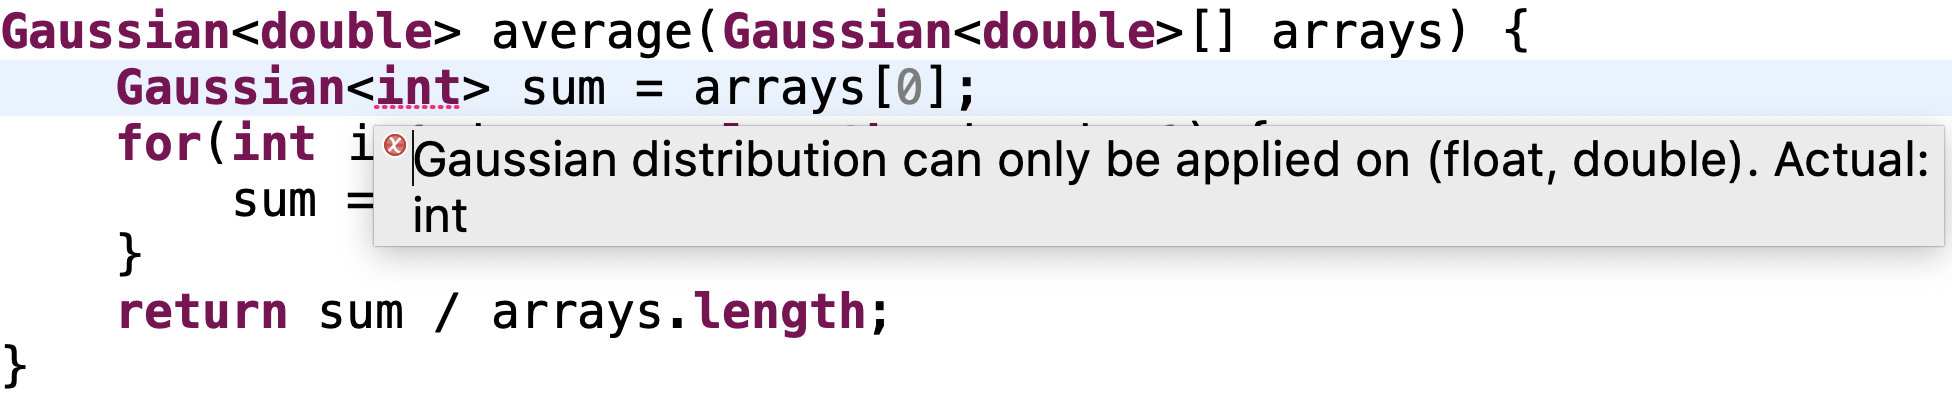
\includegraphics[width=0.6\linewidth]{img/motivation/aintea-overview}
%	\caption{Overview of the language proposed, \languageName{}}
%	\label{fig:motivation-aintea-overview}
%\end{figure}
\section[Long-term actions]{\Gls{longTermAct}}
\label{sec:example:tkm}


\subsection{Motivation}
\label{sec:tkm:intro:motiv}

\subsubsection{Delayed action}
\label{sec:tkm:intro:motiv:delayed_action}

In this section, we motivate the need to reason over delayed actions.
To do so, we first give four examples of these actions.
Then we detail why the effects of actions should be considered.
Finally, we summarise and motivate the need for incorporating actions and their effects on the knowledge. 

\paragraph{Delayed action examples}
Until here, we have claimed that adaptation processes should handle delayed actions.
In order to show their existence, we give four different examples: two based on our use case, one on cloud infrastructure and a last one on smart homes.
From our understanding, three phenomena can explain this delay: the time to execute an action(s) (Example 1), the time for the system to handle the new configuration (Example 3) and the inertia of the measured element (Example 2 and 4).

\subparagraph{Example 1: Modification of fuse states in smart grids}
Even if the Luxembourg power grid is moving to an autonomous one, not all the elements can be remotely controlled.
One example is fuses that still need to be open or closed by a human.
Open and close actions in the Luxembourg smart grid both imply technicians who are contacted, drive to fuse places and manually change their states.
If several fuses need to be changed due to one decision, only one technician will drive to them, sequentially, and executes the modifications.
For example, in our case, our industrial partner asks us to consider that each fuse modification takes 15 min whereas any incident should be detected in the minute.
Let's imagine that an incident is detected at 4 p.m. and can be solved by modifying three fuses.
The incidents will be seen as resolved by the adaptation process at 4 p.m. + 15 min * 3 = 4:45 p.m.
In this case, the delay of the action is due to the execution time that is not immediate.

\subparagraph[Example 2: Reduction of amps limits in smart grids]{Example 2: Reduction of amps limit in smart grids\footnote{This example is based on randomly generated data. As this action is not yet available on the Luxembourg smart grid, we miss real data. However, it reflects an hypothesis shared with our partner.}}
\begin{figure}
	\centering
	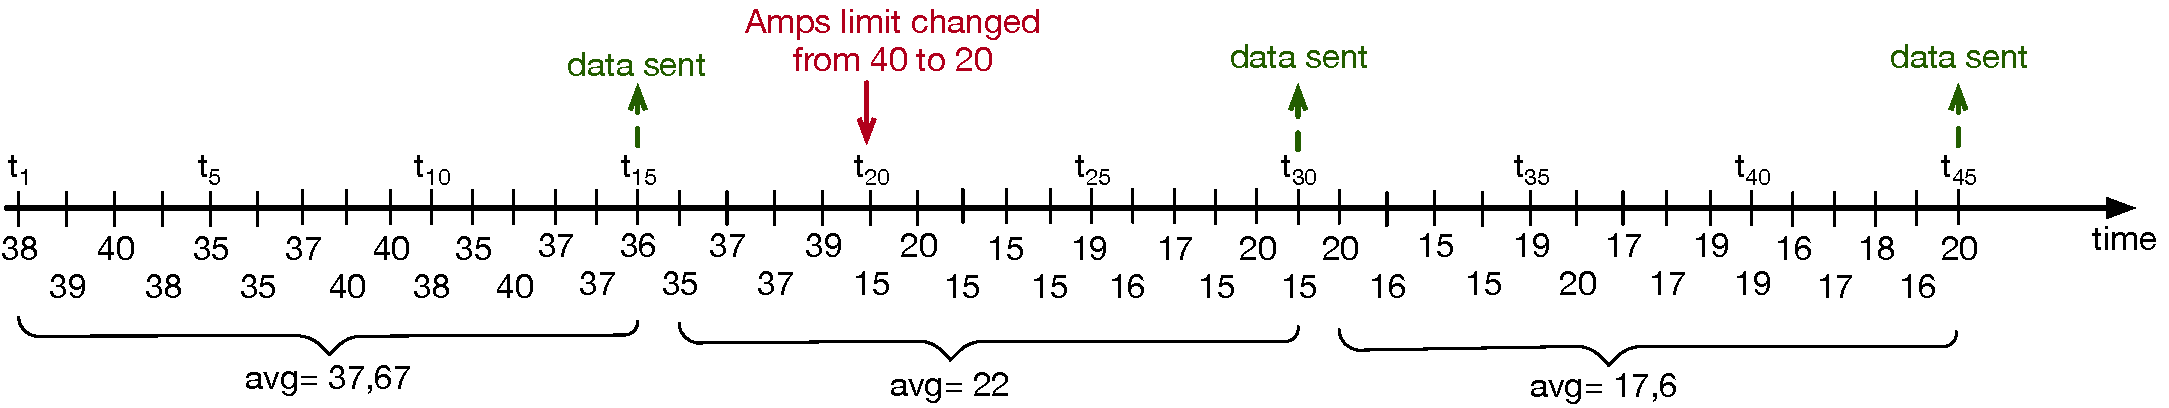
\includegraphics[width=\linewidth]{img/chapt-tkm/intro/long-action-amps-limit}
	\caption{Example of consumption measurement before and after a limitation of amps has been executed at $t_{20}$.}
	\label{fig:tkm:intro:example-long-action-amps-limit}
\end{figure}

In its smart grid project, \creos envisages controlling remotely amps limits of customers.
Customers will have two limits: a fixed one, set at the beginning, and a flexible one, remotely managed.
The action to remotely change amps limits will be performed through specific plugs, such as one for electric vehicles.
Even if the action is near instant, due to how power consumption is collected, its impacts would not be visible immediately.
Indeed, data received by \creos corresponds to the total energy consumed since the installation.
From this information, only the average of consumed data for the last period can be computed.

In Figure~\ref{fig:tkm:intro:example-long-action-amps-limit}, we depict a scenario that shows the delay between the action is executed and the impacts are measured.
Each time point represents one minute, with the consumption at this moment.

Let's imagine a customer who has his or her limit set to 40 amps\footnote{The user cannot consume more than 40 amps at a precise time $t_i$.} and consumes near this limit.
We consider that data are sent every 15 min.
After receiving data sent $t_{15}$ and processing them, the adaptation process detects an overload and decides to reduce the limits to 20 amps for the customer.
However, considering the delay for data to be collected and the one to send data\footnote{Reminder: the smart grid is not built upon a fast network such a fiber network.}, the action is received and executed at $t_{20}$.
At $t_{30}$, new consumption data is sent, here equals 22 amps.
Here, there are two situations.
First, this reduction was enough to fix the overload.
Even in this idealistic scenario, the adaptation process must wait at worst 15 min ($t_{30}$ - $t_{15}$) to see the resolution (without considering the communication time).
Second, this reduction was not enough - as the adaptation process considered that the consumption data will be at worst 20 amps and here it is 22.
Before seeing the incident as solved and knowing that the decision fixed the incident, the adaptation process should wait for new data, sent at $t_{45}$, \ie around 30 min ($t_{45} - t_{15}$) after the detection.

In this case, the delay of this action can be explained by the inertia in the average of the consumption.

\subparagraph{Example 3: Switching off a machine from a load balancer}
\begin{figure}
	\centering
	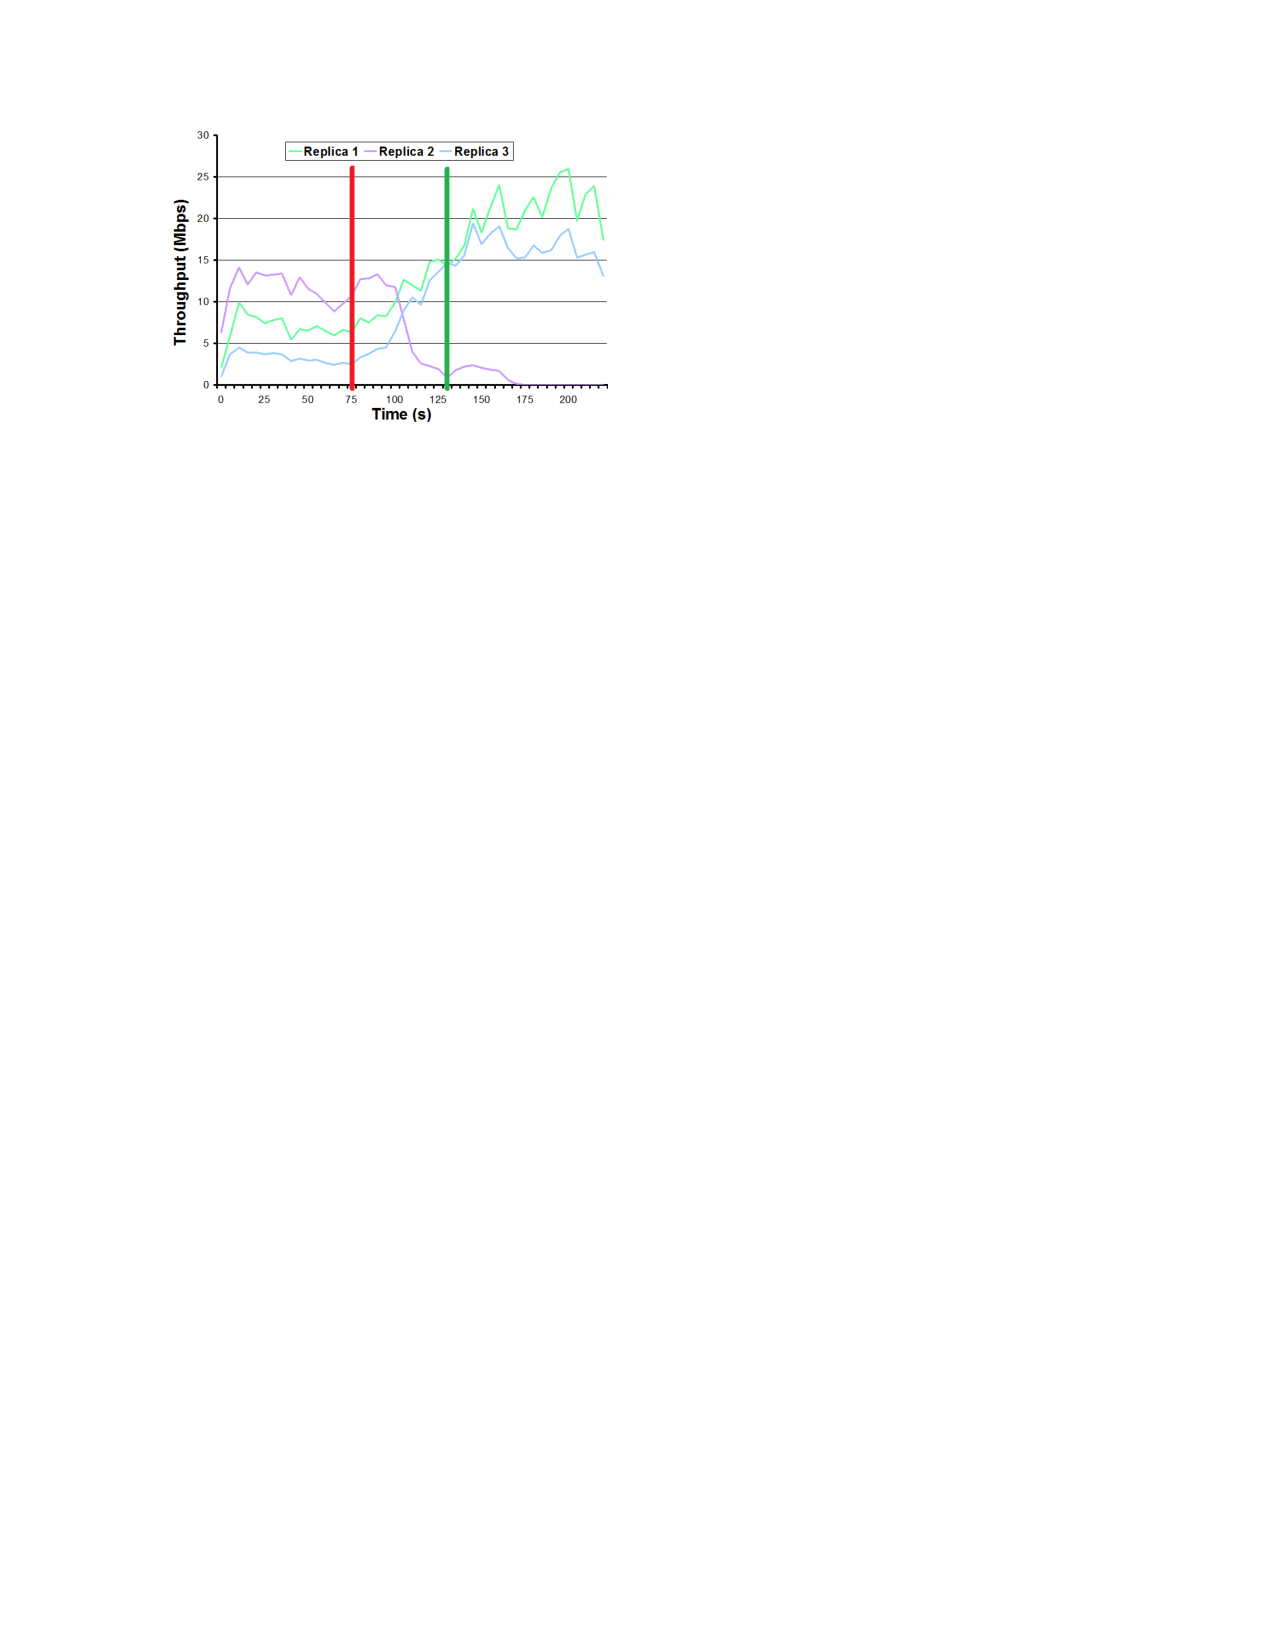
\includegraphics[width=0.5\linewidth]{img/chapt-tkm/intro/load-balencer}
	\caption{Figure extracted from~\cite{DBLP:conf/nsdi/WangBR11}. The red bar depicted the moment when Replica 2 stop receiving new connections. The green one represents the moment where all the rules in the load balancer stop considering R2. Despite these two actions, the throughput of the machine does not drop to 0 due to existing and active connections.}
	\label{fig:tkm:intro:example-load-balencer}
	
\end{figure}


An example based on cloud infrastructure of delayed actions is to remove a machine from a load balancer, for example during a scale down operation.
Scale down operations allows cloud managers to reduce allocated resources for a specific task.
It is used either to reduce the cost of the infrastructure or to reallocate them to other tasks.
In~\cite{DBLP:conf/nsdi/WangBR11}, Wang~\etal present a load-balancing algorithm.
In their evaluation, they present the figure depicted in Figure~\ref{fig:tkm:intro:example-load-balencer} that shows the evolution of the throughput after the server Replica 2 (R2) is removing from the load balancer.
The red bar shows the moment where R2 stop receiving new connection and the green the moment where it is removed from the load balancer algorithm.
However, despite these actions have been taken, R2 should finish the ongoing tasks that it is executing.
This explains why the throughout is progressively decreasing to 0 and there is a delay of around 100s between the red bars and the moment where R2 stop being active.

This example shows a delayed action due to the time required by the system to handle the new configuration.

\subparagraph{Example 4: Modifying home temperature through a smart home system}
Smart home systems have been implemented in order to manage remotely a house or to perform automatically routines.
For example, it allows users to close or open blinds from their smartphones.
Based on instruction temperatures, smart home systems manage the heating or cooling system to reach them at the desired time.
However, heating or cooling a house is not immediate, it can take several hours before the targeted temperature is reached.
Plus, if the temperature sensor and the heating or cooling system are not placed nearby, the new temperature can take time before being measured.
This can be explained due to the temperature inertia plus the delay for the temperature to be propagated.

\bigskip

Through these four examples, we show that delayed actions can be found in different kinds of systems, from CPS to cloud infrastructure.
However, not only knowing that an action is running is important but also knowing its expecting effect.
We detail this point in the following section.

\paragraph{The need to consider effects}
In the previous section, we show the existence of delayed actions.
One may argue that action statuses are already integrated into the knowledge.
For example, the OpenStack Watcher framework stores them in a database\footnote{\url{https://docs.openstack.org/watcher/latest/glossary.html\#watcher-database-definition}}, accessible through an API.
However, for the best of our knowledge Watcher does not store the expecting effects of each action.
While the adaptation process knows what action is running, it does not know what it should expect from them.

Considering our example based on the modification of fuses, if the system knows that the technician is modifying fuse states, it does not know what would be the effects.
In this case, when the adaptation process analyses the system context it may wonder: what will be the next grid configuration? How the load will be balanced? Will the future configuration fix all the current incidents?
If the effects are not considered by the adaptation process, then it may take suboptimal decisions.

Let's exemplify this claim through a scenario based on the fuse example (\cf Example 1).
As explained before, the overload detected at 4 p.m. takes around 45 min to be fixed.
The system marks this incident as \textquote{being resolved}.
In addition to this information, the knowledge contains another one saying that it is being solved by modifying three fuses.
However, during the resolution stage, a cable is also being overloaded.
The adaptation process has two solutions.
It can either wait for the end of the resolution of the first incident to see if both overloaded elements will be fixed or it takes other actions without considering the ongoing actions and their impacts.
Applying the first strategy may make the resolution of the second incident late, whereas the second one may generate a suboptimal sequence of actions.
For example, the second modifications may undo what has been done before or both actions may be conflicting.

\paragraph{Conclusion}
Actions, like fuse modification in a smart grid or removing a server from a load balancer, generated during by adaptation processes could take time upon completion. 
Moreover, the expected effects resulting from such action is reflected in the context representation only after a certain delay. 
One used workaround is the selection, often empirically, of an optimistic time interval between two iterations of the MAPE-K loop such that this interval is bigger than the longest action execution time.
However, the time to execute an action is highly influenced by system overload or failures, making such empirical tuning barely reliable.
We argue that by enriching context representation with support for past and future planned actions and their expected effects over time, we can highly enhance reasoning processes and avoid empirical tuning.

The research question that motivates our work is thus: how to enable reasoning over unfinished actions and their expected effects?

Fined and rich context information directly influences the accuracy of the actions taken.
Various techniques to represent context information have been proposed; among which we find the models@run.time~\cite{DBLP:journals/computer/MorinBJFS09, DBLP:journals/computer/BlairBF09}.
The models@run.time \linebreak paradigm inherits model-driven engineering concepts to extend the use of models not only at design time but also at runtime. 
This model-based representation has proven its ability to structure complex systems and synthesize its internal state as well as its surrounding environment.

\subsubsection{Diagnosis support}

Faced with growingly complex and large-scale software systems (e.g. smart grid systems), we can all agree that the presence of residual defects becomes unavoidable~\cite{DBLP:conf/icse/BarbosaLMJ17, DBLP:conf/icse/MongielloPS15, DBLP:conf/icse/HassanBB15}. 
Even with a meticulous verification or validation process, it is very likely to run into an unexpected behaviour that was not foreseen at design time. Alone, existing formal modelling and verification approaches may not be sufficient to anticipate these failures~\cite{DBLP:conf/icse/TaharaOH17}. 
As such, complementary techniques need to be proposed to locate the anomalous behaviour and its origin in order to handle it in a safe way.

As there might be many probable causes behind an abnormal behaviour, developers usually perform a set of diagnosis routines to narrow down the scope or origin of the failure. One way to do so is by investigating the satisfaction of its requirements and the decisions that led to this system state, as well as their timing~\cite{DBLP:conf/iceccs/BencomoWSW12}.  
In this perspective, developers may set up a set of systematic questions that would help them understand why and how the system is behaving in such a way.
These questions may comprise: 
\begin{itemize}
   \item what goal(s) the system was trying to reach by executing a tactic $a$? 
   \item what were the circumstances used by a decision $d$ and its expected impact on the context?
   \item what decision(s) influenced the system's context at a time $t$? 
\end{itemize}

Bencomo~\etal~\cite{DBLP:conf/iceccs/BencomoWSW12} argue that comprehensive explanation about the system behaviour contributes drastically to the quality of the diagnosis, and eases the task of troubleshooting the system behaviour.
To enable this, we believe that adaptive software systems should be equipped with traceability management facilities to link the decisions made to their \textbf{(i) circumstances, that is to say, the history of the system states and the targeted requirements, and (ii) the performed actions with their impact(s) on the system}.
In particular, an \textbf{adaptive system should keep a trace of the relevant historical events}.
Additionally, it should be able to \textbf{trace the goals intended to be achieved by the system to the adaptations and the decisions that have been made, and vice versa}. 
Finally, in order to enable developers to interact with the system in a clear and understandable way, appropriate abstraction to \textbf{enable the navigation of the traces and their history should also be provided}.
Unfortunately, suitable solutions to support these features are under-investigated. 

Existing approaches~\cite{hassel13,DBLP:conf/models/HeinrichSJRMHRP14,DBLP:conf/icac/EhlersHWH11,DBLP:conf/icse/MendoncaAR14,DBLP:conf/icse/CasanovaGSA14,DBLP:conf/icse/IftikharW14a} are accompanied by built-in monitoring rules and do not allow to interact with the underlying system in a simple way. 
Moreover, they do not keep track of historical changes as well as causal relationships linking requirements to their corresponding adaptations. Only flat execution logs are stored. 

\subsection{Use case scenario}
\label{sec:tkm:intro:uc}

\begin{figure}
	\centering
	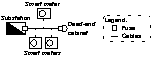
\includegraphics[width=0.5\linewidth]{img/chapt-tkm/formalism/excerptSG}
	\caption{Simplified version of a smart grid}
	\label{fig:tkm:excerptSG}
\end{figure}

In order to provide a readable and understandable example of the formalism, we give a simplified version of the use case presented in Section~\ref{sec:intro:use-case}.

\paragraph{Excerpt of a smart grid}
Figure~\ref{fig:tkm:excerptSG} shows a simplified version of a smart grid with one substation, one cable, three smart meters and one dead-end cabinet.
Both the substation and the cabinet have one fuse each.
The meters regularly send consumption data at the same timestamp.
For this example, we consider one requirement: minimizing the number of overloads.
To achieve so, among the different actions, two actions are taken into account in this example: decreasing or increasing the amps limits of smart meters.

\paragraph{Adaptation scenario}
The system starts at $t_0$ with the actions, the requirements and all element of the context that remain fixed: the grid installation.
Meters send their values at $t_1$, $t_2$ and $t_3$.
Based on these data, the load on cables and substation is computed.
On $t_1$, an overload is detected on the cable, which breaks the requirement.
At the same time point, the system decides to reduce the load of all smart meters.
The impact of these actions will be measured at $t_2$ and $t_3$, \ie the consumption will slowly reduce until the cable is no longer overloaded from $t_3$.

\paragraph{Diagnosis scenario}
As all adaptive systems, smart grids are prone to \linebreak failures~\cite{DBLP:conf/smartgridsec/0001FKNT14}.
Using our approach, an engineer could diagnose the system, and determine the adaptation process responsible for this failure. 
For instance, considering some reports about regular power cuts during the last couple of days, in a particular area, a stakeholder may want to interrogate the system and determine what past decision(s) have led to this suboptimal state.
More concretely, he will ask: did the system make any decisions that could have impacted the customer consumption? 
If so, what goal(s) the system was trying to reach and what were the values used at the time the decision(s) was(were) made?